% Preamble
\documentclass{aastex631}
\usepackage{natbib}
\usepackage{latexsym}
\usepackage{graphicx}
\usepackage{epsfig}
\usepackage{amssymb}
\usepackage{amsmath}
\usepackage{epstopdf}
\usepackage{hyperref}

%%%% Custom commands
\newcommand{\gradrad}{\ensuremath{\nabla_{\rm{rad}}}}
\newcommand{\gradad}{\ensuremath{\nabla_{\rm{ad}}}}
\newcommand{\justgrad}{\ensuremath{\nabla}}
\newcommand{\delp}{\ensuremath{\delta_{\rm{p}}}}
\newcommand{\Fbot}{\ensuremath{F_{\rm{bot}}}}
\newcommand{\Ftot}{\ensuremath{F_{\rm{tot}}}}
\newcommand{\Frad}{\ensuremath{F_{\rm{rad}}}}
\newcommand{\Fconv}{\ensuremath{F_{\rm{conv}}}}
\newcommand{\Fcz}{\ensuremath{F_{\rm{cz}}}}
\newcommand{\mP}{\ensuremath{\mathcal{P}}}
\newcommand{\mD}{\ensuremath{\mathcal{D}}}
\newcommand{\dP}{\ensuremath{\delta_{\rm{p}}}}
\newcommand{\Lcz}{\ensuremath{L_{\rm{cz}}}}
\newcommand{\mR}{\ensuremath{\mathcal{R}}}
\newcommand{\mS}{\ensuremath{\mathcal{S}}}
\newcommand\Pran{\ensuremath{\mathrm{Pr}}}
\newcommand{\brunt}{Brunt-V\"{a}is\"{a}l\"{a}}

\newcommand{\angles}[1]{\langle #1 \rangle}
\newcommand{\pd}[1]{\partial_{#1}}
\renewcommand{\vec}[1]{\boldsymbol{#1}}
\newcommand{\M}[1]{\mathbf{#1}}
\renewcommand{\dot}{\vec{\cdot}}
\renewcommand{\bar}[1]{\overline{#1}}
\newcommand{\grad}{\vec{\nabla}}
\newcommand{\cross}{\vec{\times}}
\newcommand{\laplacian}{\nabla^2}

%%%% Journal preamble
\received{}
\revised{}
\accepted{}
\published{}
\submitjournal{ApJ}

\shorttitle{Convective Penetration}
\shortauthors{Anders et al}


\begin{document}

%%%% Title and Abstract
\title{Convective penetration probably parameterizes convective overshoot}
\author[0000-0002-3433-4733]{Evan H. Anders}
\affiliation{CIERA, Northwestern University, Evanston IL 60201, USA}
\author[0000-0001-5048-9973]{Adam S. Jermyn}
\affiliation{Center for Computational Astrophysics, Flatiron Institute, New York, NY 10010, USA}
\author[0000-0002-7635-9728]{Daniel Lecoanet}
\affiliation{CIERA, Northwestern University, Evanston IL 60201, USA}
\affiliation{Department of Engineering Sciences and Applied Mathematics, Northwestern University, Evanston IL 60208, USA}
\author[0000-0001-8935-219X]{Benjamin P. Brown}
\affiliation{Department Astrophysical and Planetary Sciences \& LASP, University of Colorado, Boulder, CO 80309, USA}

\correspondingauthor{Evan H. Anders}
\email{evan.anders@northwestern.edu}

\begin{abstract}
Convection is a crucial heat transport and dynamical excitation mechanism in stars.
Parameterizations like mixing length theory adequately describe bulk convective flows, but the behavior of convective motions near convective boundaries are not well understood.
In this paper we examine how convective motions mix the background thermodynamic profiles and in turn extend the size of the convection zone, a process referred to as convective penetration.
We use a simplified Boussinesq model of stellar convection with a radiative flux.
We derive a ``penetration parameter'' $\mathcal{P}$ which compares how drastically the radiative gradient deviates from the adiabatic gradient on either side of the convective boundary.
Following \citet{roxburgh1989} and \citet{zahn1991}, we derive a parameterization in which the size of the convection zone is set by $\mP$ and the energy dissipation.
We perform 3D numerical simulations using Dedalus and find good agreement with this theory.
In stellar contexts, we expect $\mathcal{P} \approx 1$ and in this regime our results suggest that convection zones may extend beyond the Schwarzschild boundary by some 20-30\% of a mixing length.
We present a MESA solar model which uses our parameterization of convective penetration, and find that the base of the solar convection zone extends by (X amount for some choice of parameters).
We briefly discuss future experiments which could verify and extend these results to stellar contexts.
\end{abstract}
\keywords{UAT keywords}



%%%% Body of paper
\section{Introduction}
\label{sec:introduction}
Convection is a crucial heat transport mechanism in stars \citep{woosley_etal_2002, hansen_etal_2004, christensen-dalsgaard_2021}, and convective dynamics influence many poorly-understood stellar phenomena.
For example, convection drives the magnetic dynamo of the Sun, leading to the host of emergent phenomena known as solar activity \citep{brun_browning_2017}.
Convection also mixes stars compositionally, which can modify observed surface abundances or inject additional fuel into convective cores, thereby extending stellar lifetimes \citep{salaris_cassisi_2017}.
Furthermore, convective motions excite waves, which can be observed and used to constrain the thermodynamic structure of stars \citep{aerts2010, basu2016}.
A complete and nuanced understanding of convection is therefore crucial for understanding stellar structure, evolution, and observations.

Despite decades of study, robust parameterizations for the mechanisms broadly referred to as ``convective overshoot'' remain elusive, and improved parameterizations could resolve many discrepancies between observations and structure models.
In the stellar structure literature, ``convective overshoot'' refers to any convectively-driven mixing which occurs beyond the boundaries of the unstable convection zone.
This mixing can influence, for example, observed surface lithium abundances in the Sun and solar-type stars which align poorly with models \citep{pinsonneault1997, carlos_etal_2019, dumont_etal_2021}.
Furthermore, modern spectroscopic observations suggest a lower solar metallicity than previously thought, and models computed with modern metallicity estimates and opacity tables have shallower convection zones than helioseismic observations suggest \citep{basu_antia_2004, bahcall_etal_2005, vinyoles_etal_2017, asplund_etal_2021}; modeling and observational discrepancies can be reduced with additional mixing below the convective boundary \citep{christensen-dalsgaard_etal_2011}.
There is also ample evidence from massive stars with core convection that currently-employed prescriptions of convective overshoot are inadequate \citep{claret_torres_2018, jermyn_etal_2018, viani_basu_2020, martinet_etal_2021, pedersen_etal_2021}.
Since core convective overshoot increases the reservoir of fuel available for nuclear fusion at each stage in stellar evolution, improved models of core convective boundary mixing could have profound impacts on the post-main sequence evolution and remnant formation of massive stars \citep{farmer_etal_2019, higgins_vink_2020}.
In order to ensure that models can be evolved on fast (human) timescales, 1D stellar evolution codes rely on simple parameterizations of convection \citep[e.g., mixing length theory,][]{bohm-vitense1958} and convective overshoot \citep{shaviv_salpeter_1973, maeder1975, herwig2000, paxton_etal_2011, paxton_etal_2013, paxton_etal_2018, paxton_etal_2019}.
While some preliminary work has been done to couple 3D dynamical convective simulations with 1D stellar evolution codes \citep{jorgensen_weiss_2019}, these calculations are currently prohibitively expensive to perform e.g., at every timestep in a stellar evolution calculation.
In short, in order to resolve many of the discrepancies between current stellar evolution models and observations, we must come to a more complete, and \emph{parameterizeable} understanding of the manner in which convective motions extend beyond convective boundaries.

The mechanisms referred to as ``convective overshoot'' in the stellar literature fall into two hydrodynamical classes.
The first class is, confusingly, also called ``\emph{convective overshoot}'' in the fluid dynamics literature and refers to motions which extend beyond the convective boundary and mix chemical compositions but importantly do not adjust the thermodynamic profile.
The second class is called ``\emph{convective penetration},'' and refers to convective motions which mix the thermodynamic profiles beyond the convective boundary, thereby extending the adiabatically-mixed convective region.
We will follow a deep history \citep{zahn1991, brummell_etal_2002, korre_etal_2019} and use this terminology; the primary focus of this work is convective penetration.

Convective overshoot and penetration have been studied in the laboratory and through numerical simulations for decades, and the state of the field has been regularly reviewed \citep[e.g.,][]{marcus_etal_1983, zahn1991, browning_etal_2004, rogers_etal_2006, viallet_etal_2015, korre_etal_2019}.
One parameter which is commonly linked to penetration or overshoot is the ``stiffness'' of the radiative-convective interface; the stiffness is a ratio which states how stable a radiative zone is compared to an adjacent convection zone according to some measure like a dynamical frequency or characteristic entropy gradient.
Experiments and simulations exhibiting extensive convective penetration in water or other simplified, Boussinesq setups have a long history \citep{ musman1968, deardorff_etal_1969, moore_weiss_1973}.
Some of these recent simplified studies suggest that the penetration depth is highly dependent on the stiffness of the radiative-convective interface \citep{couston_etal_2017, toppaladoddi_wettlaufer_2018}, and some find very little penetration but significant stiffness-dependent overshoot \citep{korre_etal_2019}.
Some studies in density-stratified or fully compressible, stratified systems \citep[e.g.,][]{hurlburt_etal_1986, saikia_etal_2000} also found significant penetration depths, with multiple authors finding results suggesting that both penetration and overshoot depths were determined by the stiffness \citep{hurlburt_etal_1994, singh_etal_1995, browning_etal_2004, dietrich_wicht_2018}.
However, some studies have contradicted these results, showing little to no dependence on the stiffness \citep{brummell_etal_2002, rogers_glatzmaier_2005}.
Many modern simulations utilize stellar structure models as background states and find significant convective overshoot and/or penetration \citep{browning_etal_2004, rogers_etal_2006, kitiashvili_etal_2016, brun_etal_2017, pratt_etal_2017, higl_etal_2021}.
This host of experiments indeed suggests that convective penetration is \emph{probably} a process that happens in stars, but no clear model has emerged which explains whether convective penetration depends on stiffness or some other quantity.

A few flux-based theories of convective penetration have been historically considered.
\citet{roxburgh1978, roxburgh1989, roxburgh1992, roxburgh1998} derived an ``integral constraint'' from the energy conservation equation and found that the integral of the flux over the full convective and penetrative region must be balanced by the dissipation of energy on small scales, which places an upper limit on the depth of the penetrative region.
\citet{zahn1991} theorized that convective penetration should depend only on how steeply the radiative temperature gradient varies at the convective boundary.
Following \citet{zahn1991}'s work, \citet{rempel2004} derived a semianalytic model and suggested that inconsistencies seen in simulations of penetrative dynamics can be explained by the magnitude of the fluxes or luminosities driving the simulations.
Indeed, some simulations have tested this exact idea, and found that penetration depths depend strongly on the input flux \citep{singh_etal_1998, kapyla_etal_2007, tian_etal_2009, hotta2017, kapyla2019}.
Furthermore, in the limit of low stiffness, the simulations of \citet{hurlburt_etal_1994} and \citet{rogers_etal_2006} seem to agree with Zahn's theory (although at high stiffness they disagree).
In light of these results, and the possible importance of fluxes, Roxburgh's integral constraint and Zahn's theory deserve to be revisited.

In this work, we design two numerical experiments to test \citet{zahn1991}'s idea that the penetration depth depends on the shape of the radiative gradient at the convective boundary.
We use a modified incompressible, Boussinesq model to study the simplest possible system, and use \citet{roxburgh1989}'s constraint to derive a theory analogous to \citet{zahn1991}'s in this simplified limit.
\begin{quote}
\emph{
We find that the extent of convective penetration depends strongly on the shape and magnitude of the radiative gradient near the convective boundary.
}
\end{quote}
Thus, the penetration depth can be calculated using the radiative conductivity (or opacity) around the convective boundary.

We present these findings as follows.
In Sec.~\ref{sec:theory}, we describe our modified Boussinesq equations, derive a theory of convective penetration similar to \citet{zahn1991}'s, and retrieve predictions for our two experimental designs from that theory.
In Sec.~\ref{sec:simulation_details}, we describe our simulation setup and parameters.
In Sec.~\ref{sec:results}, we present the results of these simulations, with a particular focus on the depth of the penetrative regions.
In Sec.~\ref{sec:solar_model}, we create and discuss a solar MESA model which uses this theory to determine the bottom of the solar convection zone.
Finally, we discuss how future simulations can put finer constraints on this theory in Sec.~\ref{sec:discussion}.

\section{Theory}
\label{sec:theory}

\subsection{Equations \& flux definitions}
\label{sec:theory_equations}
Throughout this work, we will utilize a modified version of the incompressible Boussinesq equations of motion,
\begin{align}
&\grad\dot\vec{u} = 0 
\label{eqn:incompressible} \\
&\partial_t \vec{u} + \vec{u}\dot\grad\vec{u} = -\frac{1}{\rho_0}\grad p + \frac{\rho_1}{\rho_0}\vec{g} + \nu\grad^2 \vec{u} 
\label{eqn:momentum} \\
&\partial_t T + \vec{u}\dot\grad T + w \gradad + \grad\dot[-k \grad \overline{T}] = \chi\grad^2 T' + Q
\label{eqn:temperature} \\
&\frac{\rho_1}{\rho_0} = -|\alpha| T.
\label{eqn:boussinesq}
\end{align}
Here, the density is decomposed into a constant background $\rho_0$ with fluctuations $\rho_1$ which appear only in the buoyancy force and depend on the temperature $T$ and the coefficient of thermal expansion $\alpha = \partial\ln\rho / \partial T$.
We furthermore define the velocity vector $\vec{u}$, the viscous diffusivity $\nu$, the thermal diffusivity $\chi$, the bulk internal heating $Q$ \citep[similar but not identical to that studied by e.g.,][]{goluskin_vanderpoel_2016}, and the adiabatic temperature gradient $\gradad$.
We define $\gradad$ as a positive value to align with stellar structure conventions; thus marginal stability is achieved when $\partial_z T = -\gradad$.
We will consider Cartesian coordinates $(x, y, z)$ with a constant vertical gravity $\vec{g} = -g\hat{z}$.
The equations we use are similar to those derived by \citet{spiegel_veronis_1960} and utilized by e.g., \citet{korre_etal_2019}, but we allow the mean temperature profile $\overline{T}$ to carry a radiative flux $\Frad = -k \grad \overline{T}$, where $k$ is a radiative diffusivity which can vary with height.
The classic thermal diffusion term $\chi \grad^2 T'$ therefore carries no average flux and acts only on the fluctuations away from the mean temperature profile, $T' \equiv T - \overline{T}$; throughout this work, we will represent horizontal averages with bars ($\overline{\,\cdot\,}$) and fluctuations away from those averages with primes ($'$).
Finally, we will assume a model in which an unstable convection zone sits below a stable radiative zone, but the same logic applies to the inverted problem.

Assuming convection reaches a time-stationary state, we horizontally-average and vertically integrate Eqn.~\ref{eqn:temperature} to find
\begin{equation}
\overline{\Ftot} = \overline{\Frad} + \overline{\Fconv} = \int Q dz + \Fbot,
\label{eqn:flux_definition}
\end{equation}
where $\Fbot$ is the flux carried at the base of the convection zone, and $\overline{\Ftot}$ is the total flux, which can vary in height due to the heating $Q$.
We note that $k$ and the temperature gradient $\justgrad \equiv -\partial_z \bar{T}$ fully specify $\Frad$ and in turn the convective flux, $\bar{\Fconv} = \bar{\Ftot} - \bar{\Frad}$.
We define the radiative gradient 
\begin{equation}
\gradrad = \frac{\bar{\Ftot}}{k}
\label{eqn:gradrad_definition}
\end{equation}
and note that the classical Schwarzschild boundary of the convection zone is the height $z = L_s$ at which $\gradrad = \gradad$ and $\bar{\Fconv} = 0$.

\subsection{Kinetic energy \& the dissipation-flux link}
\label{sec:theory_energy}
\begin{figure}[t!]
\centering
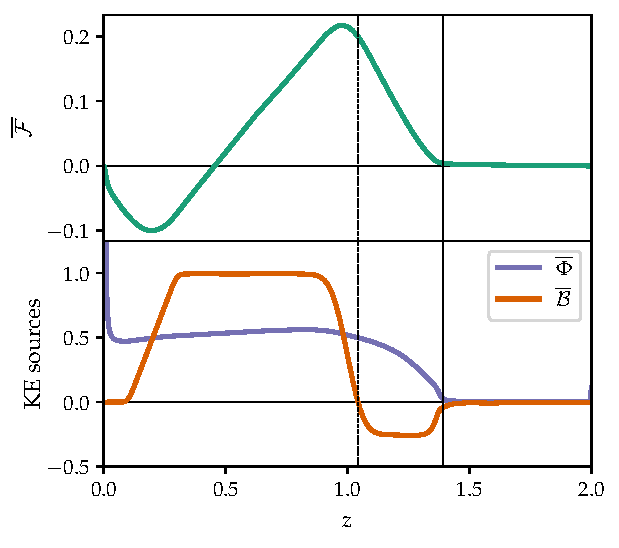
\includegraphics[width=\textwidth]{theory_profiles.pdf}
\caption{
(left) The vertical profile of the kinetic energy fluxes $\mathcal{F}$.
This profile goes to zero at the bottom boundary, again at the dashed line, and at the top of the PZ near $z \approx 1.5$; Eqn.~\ref{eqn:integral_constraint} holds between any two of these points.
(middle) the evolved value of $\justgrad$ (green) compared to $\gradad$ (grey) and $\gradrad$ (red); note the extended penetration zone where $\justgrad \approx \gradad > \gradrad$.
(right) Source terms from Eqn.~\ref{eqn:kinetic_energy_1D} normalized by the maximum of $\overline{\mathcal{B}}$.
\label{fig:theory_profiles}
}
\end{figure}

Taking an inner product of the velocity and Eqn.~\ref{eqn:momentum} reveals the kinetic energy equation,
\begin{equation}
\frac{\partial \mathcal{K}}{\partial t}
+ \grad\dot\mathcal{F}
= \mathcal{B} - \Phi,
%\frac{\partial}{\partial t}\left(\frac{|\vec{u}|^2}{2}\right) 
%+ \grad\dot\left[\vec{u}\left(\frac{|\vec{u}|^2}{2} + \frac{p}{\rho_0}\right) - \nu\vec{u}\cross\vec{\omega}\right]
%= |\alpha| g w T - \nu|\vec{\omega}|^2,
\label{eqn:kinetic_energy}
\end{equation}
where we define the kinetic energy $\mathcal{K} \equiv |\vec{u}|^2/2$, the fluxes of kinetic energy $\mathcal{F} \equiv \left[\vec{u}(\mathcal{K} + p/\rho_0) - \nu\vec{u}\cross\vec{\omega} \right]$, the buoyant energy generation rate $\mathcal{B} \equiv |\alpha| g w T'$, and the viscous dissipation rate $\Phi \equiv \nu |\vec{\omega}|^2$ where $\vec{\omega} = \grad\cross\vec{u}$ is the vorticity and $|\vec{u}|^2 = \vec{u}\dot\vec{u}$ \& $|\vec{\omega}|^2 = \vec{\omega}\dot\vec{\omega}$.
We next take a horizontal- and time-average of Eqn.~\ref{eqn:kinetic_energy} (which we will represent with $\bar{\,\cdot\,}$ for simplicity).
Assuming that $\bar{\mathcal{K}}$ reaches a statistically stationary state, convective motions satisfy
\begin{equation}
\frac{d\bar{\mathcal{F}}}{dz} = \bar{\mathcal{B}} - \bar{\Phi}.
\label{eqn:kinetic_energy_1D}
\end{equation}
It is reasonable to assume that $\mathcal{F}$ is zero at the boundaries of the convecting region (see Fig.~\ref{fig:theory_profiles}, left panel).
We integrate Eqn.~\ref{eqn:kinetic_energy_1D} vertically between these zeros of the flux to find
\begin{equation}
\int \bar{\mathcal{B}}\,dz = \int \bar{\Phi}\,dz.
\label{eqn:integral_constraint}
\end{equation}
Integral constraints of this form are the basis for a broad range of analyses in Boussinesq convection \citep[see e.g.,][]{ahlers_etal_2009, goluskin2016} and were considered in the context of penetrative convection by \citet{roxburgh1989}.
Eqn.~\ref{eqn:integral_constraint} is the straightforward statement that work by buoyancy on large scales must be balanced by viscous dissipation on small scales.
We now find it instructive to break up the convecting region into a classical ``convection zone'' (CZ) and a extended ``penetration zone'' (PZ); we will assume that convective motions are efficient in each of these zones so that $\justgrad = \gradad$ in both the CZ and PZ.
We furthermore note that the buoyant energy generation is directly proportional to the convective flux, $\bar{\mathcal{B}} = |\alpha|g\bar{w T'} = |\alpha| g \bar{\Fconv}$.
Thus, in the PZ where $\gradad > \gradrad$, we know that $\bar{\Fconv} < 0$ and so $\bar{\mathcal{B}} < 0$ too.
Breaking up Eqn.~\ref{eqn:integral_constraint}, we see that
\begin{equation}
\int_{\rm{CZ}} \bar{\mathcal{B}}\,dz \qquad=\qquad
\int_{\rm{CZ}} \bar{\Phi}\,dz + \int_{\rm{PZ}} \bar{\Phi}\,dz + \int_{\rm{PZ}}(-\bar{\mathcal{B}})\,dz.
\label{eqn:constraint_cz_pz_split}
\end{equation}
Eqn.~\ref{eqn:constraint_cz_pz_split} is thus arranged so that the (positive) buoyant engine of convection is on the left-hand side, and the (positive) sinks of energy are on the RHS.
We see that the size of the PZ is set by some combination of viscous dissipation and buoyancy breaking, whose total effect cancels out any remaining work that dissipation in the convection zone did not itself cancel.
we now find it instructive to parameterize the fraction of the buoyant engine consumed by CZ dissipation  
\begin{equation}
f \equiv \frac{\int_{\rm{CZ}} \bar{\Phi}\,dz}{\int_{\rm{CZ}}\bar{\mathcal{B}}\,dz}.
\label{eqn:f_defn}
\end{equation}
Under this parameterization, Eqn.~\ref{eqn:constraint_cz_pz_split} can be written
\begin{equation}
\frac{\int_{\rm{PZ}} \bar{\Phi}\,dz + \int_{\rm{PZ}}(-\bar{\mathcal{B}})\,dz}{\int_{\rm{CZ}} \bar{\mathcal{B}}\,dz}
= 1 - f,
\label{eqn:first_pz_parameterization}
\end{equation}
and we can immediately read off limits on a hypothetical PZ according to $f$,
\begin{enumerate}
\item In the limit that $f \rightarrow 0$, viscous dissipation is extremely inefficient.
It is probably also reasonable to assume that $\int_{\rm{PZ}}\bar{\Phi}\,dz \rightarrow 0$, and so Eqn.~\ref{eqn:first_pz_parameterization} states that the PZ must be large enough for its negative buoyant work to be equal in magnitude to the positive buoyant work of the CZ.
This is the integral constraint on the maximum size of the PZ that \citet{roxburgh1989} derived.
\item In the limit that $f \rightarrow 1$, viscous dissipation is efficient in the CZ and cancels out the work done by buoyancy.
This is the case in standard Rayleigh-B\'{e}nard convection when the convection is contained between two hard plates.
Per Eqn.~\ref{eqn:first_pz_parameterization}, the positive-definite PZ terms must approach zero and no PZ develops in this limit.
\end{enumerate}
In general, we anticipate from the results of e.g., \citet{currie_browning_2017} that $f$ is closer to 1 than 0, but its precise value must be measured directly from simulations.
Indeed, we find that $f \gg 0$ but $f < 1$ in our simulations (see e.g., Fig.~\ref{fig:theory_profiles}, right panel).

Assuming that a PZ of depth $\delp$ develops above a CZ of depth $L_{\rm{CZ}}$, we model the PZ dissipation as
\begin{equation}
\int_{\rm{PZ}} \bar{\Phi}\,dz = \xi\frac{\delp}{L_{\rm{CZ}}}\int_{\rm{CZ}}\bar{\Phi} = \xi \delp \Phi_{\rm{CZ}}.
\end{equation}
Here $\Phi_{\rm{CZ}}$ is the average dissipation value in the CZ and $\xi$ is a parameter that describes the shape of the dissipation profile as a function of height in the PZ.
In other words, we assume that $\bar{\Phi} \approx \Phi_{\rm{CZ}}$ at the CZ-PZ boundary and then falls off with height.
The shape of $\bar{\Phi}$ determines the value of $\xi$, with a linear falloff producing $\xi = 1/2$, a quadratic falloff producing $\xi = 2/3$, and the in which $\bar{\Phi}$ does not decline with height produces $\xi = 1$.
Regardless, $\xi$ is another measurable parameter bounded by $[0, 1]$. 
With this parameterization, we rewrite Eqn.~\ref{eqn:first_pz_parameterization}
\begin{equation}
-\frac{\int_{\rm{PZ}}\bar{\Fconv}\,dz}{\int_{\rm{CZ}}\bar{\Fconv}\,dz} + f\xi\frac{\delp}{L_{\rm{CZ}}}
= (1 - f).
\label{eqn:theory_fraction}
\end{equation}
In order to derive a specific prediction for the PZ depth, it is necessary to specify the vertical shape of $\overline{\Fconv}$.
We will study two cases in this work, laid out below.
In both of these cases, we will define a nondimensional ``Penetration Parameter'' whose magnitude is set by the ratio of the convective flux some equidistant length $\epsilon$ both above and below the Schwarzschild convective boundary $L_s$ (assuming the region above the boundary is an adiabatic penetrative zone),
\begin{equation}
\mP \equiv -\frac{\overline{\Fconv}(z = L_s - \epsilon)}{\overline{\Fconv}(z = L_s + \epsilon)}.
\label{eqn:theory_P_defn}
\end{equation}
Since $\Fconv < 0$ in the PZ, the sign of $\mP$ is positive.

%where $\Fconv = w T$ and angles $\angles{\,\cdot\,}$ represent a time- and volume- average.
%It may seem counterintuitive to find that the viscous energy dissipation term $\nu\angles{|\vec{\omega}|^2}$ operates on the same order of magnitude as the convective flux.
%However, Eqn.~\ref{eqn:ke_averages} is a statement of a balance between buoyant injection of energy into the system on large scales and dissipation on small scales.
%Dimensionally, the viscous dissipation term is $\nu u^2 / \ell^2$, where $u$ is the average convective velocity and $\ell$ is the length scale of velocity gradients on the dissipation scale, and it is reasonable to assume that $\ell^2 \propto \nu$ leading to an appreciable dissipation even at very small $\nu$.
%\citet{currie_browning_2017} demonstrated that even in appreciably density-stratified atmospheres, the magnitude of viscous dissipation remains large for turbulent flows, so the importance of $\nu |\vec{\omega}^2|$ is perhaps not too surprising.
%
%We now decompose the convection zone into a zone which is classically unstable according to the Schwarzschild criterion (called the CZ, with depth $L_s$) and a dynamically distinct penetrative zone (called the PZ, with depth $\delp$).
%Following Eqn.~\ref{eqn:ke_averages}, we write
%\begin{equation}
%\frac{1}{L_s + \delp}\left(\int_{\rm{CZ}} \bar{\Fconv} dz + \int_{\rm{PZ}} \bar{\Fconv} dz \right) = \frac{\nu}{|\alpha| g} \angles{|\vec{\omega}|^2}.
%\label{eqn:flux_breakup}
%\end{equation}
%Rearranging, we retrieve 
%\begin{equation}
%\frac{\int_{\rm{PZ}}\bar{\Fconv}\,dz}{\int_{\rm{CZ}}\bar{\Fconv}\,dz} = -(1 - f),
%\qquad\rm{with}\qquad
%f \equiv \frac{(L_s + \delp)}{|\alpha| g} \frac{\nu\angles{|\vec{\omega}|^2}}{\int_{\rm{CZ}} \bar{\Fconv} dz}
%= \frac{\int_{\rm{CZ+PZ}}\bar{\Fconv}\,dz}{\int_{\rm{CZ}}\bar{\Fconv}\,dz},
%\label{eqn:preliminary_flux_ratio}
%\end{equation}
%where the final equality is a tautological rearrangement of the decomposition of the flux integral in Eqn.~\ref{eqn:flux_breakup}.
%The upshot of this equation is that, if the convective dissipation $f$ is known, the size of the penetrative zone can be immediately found from simple flux arguments.
%We theorize that $f$ is some constant which weakly depends upon things like the turbulence of the flows, the stiffness of the radiative-convective interface, etc.
%If this is the case, Eqn.~\ref{eqn:preliminary_flux_ratio} represents a simple parameterization of the nature of the penetrative zone in terms of the convection zone.
%In order to derive a specific penetration depth $\delp$, we must turn to a more in-depth examination of the fluxes in the PZ.


\subsubsection{Case I: Discontinuous flux}
\label{sec:discontinuous_theory}
We first consider a model which satisfies
\begin{equation}
\overline{\Fconv}(z) = \Fcz \begin{cases}
1			&	z \leq \Lcz,\\
-\mP_D^{-1}  & 	z > \Lcz 
\end{cases}.
\end{equation}
Here, $\Fcz$ is a constant value of flux carried in the convection zone and $\mP_D$ is the penetration parameter (subscript D for discontinuous case).
Plugging this functional form of the flux into Eqn.~\ref{eqn:theory_fraction}, and integrating the CZ over a depth $L_{\rm{CZ}}$ below $L_s$ and the PZ over a depth $\delp$ above $L_s$, we predict
\begin{equation}
\frac{\delp}{L_{\rm{CZ}}} = \mP_D \frac{1 - f}{1 + \xi f \mP_D}.
\label{eqn:discontinuous_prediction}
\end{equation}
Assuming that $f$ is a weak function of $\mP_D$, we see that the size of the penetration region is roughly linearly proportional to $\mP_D$ at small $\mP_D$, but saturates due to dissipation at large $\mP_D$.
Intuitively, this result makes sense: as $\mP_D$ grows, the magnitude of $\overline{\Fconv}$ and the breaking force of buoyancy in the PZ shrink, resulting in larger penetrative regions (but this growth cannot extend indefinitely).

\subsubsection{Case II: Piecewise linear flux}
\label{sec:linear_theory}
We next assume that $\overline{\Fconv}(z)$ is not discontinuous at the CZ-PZ boundary, but that its derivative may be,
\begin{equation}
\overline{\Fconv}(z) = 
\frac{\partial \Frad}{\partial z}\bigg|_{\rm{CZ}}
\begin{cases}
(L_p - z) & z \leq L_p \\
-\mP_L^{-1} (z - L_p) & z > L_p
\end{cases},
\end{equation}
where $(\partial \Frad / \partial z)|_{\rm{CZ}}$ is a constant and $\mP_L$ is the penetration parameter (subscript L for linear case).
Again, solving Eqn.~\ref{eqn:theory_fraction} with this functional form of the flux and integrating over $L_{\rm{CZ}}$ in the CZ and $\delp$ in the PZ, we retrieve a quadratic equation.
This equation has two solution branches, only one of which corresponds to a positive value of $\delp$.
On that branch, we find
\begin{equation}
\frac{\delp}{L_p} = \sqrt{\mP_L (1 - f)} \,\,(\sqrt{\zeta^2 + 1} - \zeta),
\label{eqn:linear_prediction}
\end{equation}
where $\zeta \equiv (\xi f/2)\sqrt{\mP_L/(1-f)}$.
So we expect the penetration depth to be roughly proportional to $\sqrt{\mP_L}$ for small values of $\mP_L$, and to again saturate at large values of $\mP_L$. 

In this work, we will test the predictions of Eqns.~\ref{eqn:discontinuous_prediction} and \ref{eqn:linear_prediction}.
Our goals are to see if the predicted scalings with the penetration parameter $\mP$ are realized in simulations, and to measure the dependence of $f$ on various parameters in local simulations.

\section{Simulation Details}
We nondimensionalize Eqns.~\ref{eqn:incompressible}-\ref{eqn:boussinesq} on the length scale of the Schwarzschild-unstable convection zone $L_s$, the timescale of freefall across that convection zone $\tau_{\rm{ff}}$, and the temperature scale of the internal heating over that freefall time $\Delta T$,
\begin{equation}
\begin{split}
&T^* = (\Delta T)T = Q_0 \tau_{\rm{ff}} T,\qquad
\partial_{t^*} = \tau_{\rm{ff}}^{-1}\partial_t = \left(\frac{|\alpha| g Q_0}{L_s}\right)^{1/3} \partial_t,\qquad
\grad^* = L_s^{-1} \grad,\qquad
\vec{u}^* = u_{\rm{ff}}\vec{u} = \left(|\alpha| g Q_0 L_s^2\right)^{1/3}\vec{u},
\\
&p^* = \rho_0 u_{\rm{ff}}^2\varpi,\qquad
k^* = (L_s^2 \tau_{\rm{ff}}^{-1})k,\qquad
Q^* = Q_0 Q,\qquad
\mR = \frac{u_{\rm{ff}} L_s}{\nu},\qquad
\Pran = \frac{\nu}{\chi}.
\end{split}
\end{equation}
For convenience, here we define quantities with $*$ (e.g., $T^*$) as being the ``dimensionful'' quantities of Eqns.~\ref{eqn:incompressible}-\ref{eqn:boussinesq}.
Going forward, quantities without $*$ (e.g., $T$) will be dimensionless.
The dimensionless equations of motion are therefore
\label{sec:simulation_details}
\begin{align}
&\grad\dot\vec{u} = 0 
\label{eqn:nondim_incompressible} \\
&\partial_t \vec{u} + \vec{u}\dot\grad\vec{u} = -\grad \varpi + T \hat{z} + \mR^{-1}\grad^2 \vec{u}
\label{eqn:nondim_momentum} \\
&\partial_t T + \vec{u}\dot\grad T + w \grad_{\rm{ad}}  + \grad\dot[-k \grad \overline{T}] = (\Pran\mR)^{-1}\grad^2 T' + Q.
\label{eqn:nondim_temperature}
\end{align}
We construct a domain in the range $z \in [0, L_z]$ where in this work we choose $L_z \geq 2$ so that the domain is at least twice as deep as the Schwarzschild-unstable convection zone.
We decompose the temperature field into a time-stationary initial background and fluctuations, $T(x, y, z, t) = T_0(z) + T_1(x, y, z, t)$.
For boundary conditions, we impose impenetrable, no-slip boundary conditions at the top and bottom of the box so that $\vec{u} = 0$ at $z = [0, L_z]$.
We also impose a fixed-flux boundary at the bottom of the box ($\partial_z T_1 = 0$ at $z = 0$) and a fixed temperature boundary at the top of the domain ($T_1 = 0$ at $z = L_z$).

We impose a constant internal heating which spans only part of the convection zone,
\begin{equation}
Q = \begin{cases}
0		& z < 0.1\,\,\rm{or}\,\,z\geq 0.1 + \delta_H,\\
|Q_{\rm{mag}}|		& 0.1 \leq z \leq 0.1 + \delta_H
\end{cases}.
\label{eqn:sim_Q}
\end{equation}
The integrated value of the flux through the system from the heating is therefore $F_H = \int_0^{L_z} Q_{\rm{mag}} dz = Q_{\rm{mag}}\delta_H$.
Throughout this work we choose $Q_{\rm{mag}} = 1$ and $\delta_H = 0.2$ so $F_H = 0.2$.
We offset this heating from the bottom boundary to $z = 0.1$ to avoid heating within the bottom impenetrable boundary layer where velocities go to zero and $k$ is small; this prevents strong temperature gradients from establishing there.
We assume that the (adiabatic) temperature gradient at the bottom boundary carries some flux, $\Fbot = \zeta F_H$ and we choose $\zeta = 10^{-3}$ so that most of the flux in the convection zone is carried by the convection.

In our equations, we expect the volume-average convective velocities to depend on the magnitude of the heating, $\angles{\vec{u}} \approx Q_{\rm{mag}}^{1/2} \approx 1$, so the characteristic convective frequency is $f_{\rm{conv}} \approx \angles{\vec{u}} L_s \approx 1$.
The stiffness is defined,
\begin{equation}
\mS \equiv \frac{N^2}{f_{\rm{conv}}^2} \approx N^2,
\end{equation}
where $N^2$ is the \brunt$\,$frequency in the radiative zone.
In our nondimensionalization, $N^2 = \gradad - \gradrad$ where $\gradrad = \Ftot/k$.
We treat $\mS$ as a control parameter; by choosing a value of the stiffness we set the magnitude of the background temperature gradient, $\partial_z T_0$ which in turn sets the value of $k$ in the radiative zone.

The crucial place in which our model differs from that of prior work is that we define the ``Penetration Parameter,'' $\mP$, according to Eqn.~\ref{eqn:theory_P_defn}.
We construct our experiments so that $\mP$ and $\mS$ can be varied separately.
We suspect that many past experiments have implicitly set $\mP \approx \mS^{-1}$, and therefore found negligible penetration for moderate to high stiffness.

Aside from $\mS$ and $\mP$, the two remaining control parameters $\mR$ and $\Pran$ determine the degree of turbulence.
The value of $\mR$ roughly corresponds to the value of the peak Reynolds number $\rm{Re} = \mR |\vec{u}|$ measured in the simulations, and we set the ratio of the diffusivities $\Pran = 0.5$ throughout this work.
Astrophysical convection is in the limit of $\Pran \ll 1$ \citep{garaud2021}; we choose a modest value of $\Pran$ which slightly separates the scales between thermal and viscous structures while still allowing us to achieve convection with large Reynolds and P\'{e}clet numbers.

\subsection{Case I: Discontinuous flux}
Most of the simulations in this paper have a discontinuous convective flux at the Schwarzschild convective boundary.
We achieve this by constructing a discontinuous radiative conductivity,
\begin{equation}
k = \begin{cases}
k_{\rm{CZ}}	&	z < 1 \\
k_{\rm{RZ}} &	z \geq 1
\end{cases},
\label{eqn:sim_discontinuous_k}
\end{equation}
where CZ refers to the convection zone and RZ refers to the radiative zone (some of which will be occupied by the penetrative zone PZ).
Leaving $\mS$ and $\mP_D$ as free parameters and requiring that the adiabatic gradient can carry $\Fbot$ at $z = 0$ and that the radiative gradient can carry $F_H + \Fbot$ for $z \geq 1$ specifies this system fully,
\begin{equation}
k_{\rm{RZ}} = \frac{\delta_H}{\mS\mP_D},\qquad
k_{\rm{CZ}} = k_{\rm{RZ}}\frac{1}{1 + \zeta + \mP_D^{-1}},\qquad
\gradad = Q_{\rm{mag}}\mS\mP_D(1 + \zeta + \mP_D^{-1}),\qquad
\gradrad = \gradad - Q_{\rm{mag}}\mS.
\end{equation}

We study three sweeps through the ($\mP_D$, $\mS$, $\mR$) parameter space in this paper in which we hold two of these parameters constant and vary the other.
We use reference values of $\mP_D = 4$, $\mS = 10^3$, and $\mR = 400$; all parameter space sweeps pass through these values.
According to Eqn.~\ref{eqn:discontinuous_prediction}, we expect $\delp \propto \mP_D$.

\subsection{Case II: Piecewise linear flux}
We additionally study a select few simulations where the flux's gradient may be discontinuous at the Schwarzschild convective boundary.
We achieve this by constructing a radiative conductivity with a piecewise discontinuous gradient,
\begin{equation}
\partial_z k = \partial_z k_0
\begin{cases}
1	&	z < 1 \\
\mP_L^{-1} &	z \geq 1
\end{cases}
\label{eqn:sim_linear_k}
\end{equation}
Since $k$ varies with height, the value of $\mS$ and $\mP$ also vary with height; we specify their values at $z = 2$.
By this choice, we require
\begin{equation}
\partial_z k_0 = \frac{\delta_H}{L_s \mS \xi},\qquad
k_b = \frac{\delta_H\zeta}{\mS\xi},\qquad
\gradad = Q \mS \xi,
\end{equation}
where $\xi \equiv 1 + \mP_L(1 + \zeta)$.
In these simulations, we hold $\mS = 10^3$ and $\mR = 800$ while varying $\mP_L$.
According to Eqn.~\ref{eqn:linear_prediction}, we expect $\delta_p \propto \mP_L^{1/2}$.

\subsection{Numerics}
We time-evolve equations \ref{eqn:nondim_incompressible}-\ref{eqn:nondim_temperature} using the Dedalus pseudospectral solver \citep{burns_etal_2020}\footnote{we use commit \href{https://github.com/DedalusProject/dedalus/commit/efb13bdaa09816dde3eee897bc2a15fc284ea2f1}{efb13bd}; the closest stable release to this commit is \href{https://github.com/DedalusProject/dedalus/releases/tag/v2.2006}{v2.2006}.} using timestepper SBDF2 \citep{wang&ruuth2008} and safety factor 0.35.
All fields are represented as spectral expansions of $n_z$ Chebyshev coefficients in the vertical ($z$) direction and as ($n_x$,$n_y$) Fourier coefficients in the horizontal ($x$,$y$) directions; our domains are therefore horizontally periodic.
The aspect ratio of our domains is two so that $x \in [0, L_x]$ and $y \in [0, L_y]$ with $L_x = L_y = 2 L_z$.
To start our simulations, we add random noise temperature perturbations with a magnitude of $10^{-3}$ to a background temperature profile $\overline{T}$; we discuss the choice of $\overline{T}$ in appendix \ref{app:accelerated_evolution}.
We produce the figures in this paper using matplotlib \citep{hunter2007, mpl3.3.4}.
All of the Python scripts used to run the simulations in this paper and to create the figures in this paper are publicly available in a git repository, found at [CITE].

Spectral methods with finite coefficient expansions cannot capture true discontinuities.
In order to approximate discontinuous functions such as Eqns.~\ref{eqn:sim_Q}, \ref{eqn:sim_discontinuous_k}, and \ref{eqn:sim_linear_k}, we must use smooth transitions.
To create these smooth transitions, we define an approximate Heaviside step function using the error function,
\begin{equation}
H(z; z_0, d_w) = \frac{1}{2}\left(1 + \rm{erf}\left[\frac{z - z_0}{d_w}\right]\right).
\label{eqn:heaviside}
\end{equation}
In the limit that $d_w \rightarrow 0$, this function behaves identically to the classical Heaviside function centered at $z_0$.
While constructing Eqn.~\ref{eqn:sim_Q} and Eqn.~\ref{eqn:sim_linear_k}, we use $d_w = 0.02$; while constructing Eqn.~\ref{eqn:sim_discontinuous_k} we use $d_w = 0.075$.
In all other cases, we use $d_w = 0.05$.

\subsection{Penetration depth measurements}
In our evolved simulations, we find that the penetrative region has a nearly adiabatic stratification $\justgrad \approx \gradad$.
In order to characterize the vertical extent of the penetrative region, we measure how drastically $\justgrad$ has departed from $\gradad$.
We define the difference between the adiabatic and radiative gradient,
\begin{equation}
\Delta\justgrad \equiv \gradad(z) - \gradrad(z).
\end{equation}
We measure penetration and overshoot depths in terms of ``departure points,'' or heights at which the realized temperature gradient $\justgrad$ has evolved away from the adiabatic $\gradad$ by some fraction $h < 1$.
Specifically,
\begin{equation}
L_s + \delta_{h} = \rm{max}(z) \mid \justgrad > \gradad - h\,\Delta\justgrad.
\end{equation}
In this work, we measure the 10\% ($\delta_{0.1}$), 50\% ($\delta_{0.5}$), and 90\% ($\delta_{0.9}$) departure points.
Using \citet{zahn1991}'s terminology, $\delta_{0.1}$ is the top of the PZ while $\delta_{0.5}$ and $\delta_{0.9}$ represent the middle and top of the ``thermal adjustment layer.''
We will simply refer to these as three different measures of the top of the PZ.
We find that these measurements based on the (slowly-evolving) thermodynamic profile are more robust and straightforward than many previous dynamically-based prescriptions \citep[see e.g.,][for a nice discussion]{pratt_etal_2017}.

\section{Results}
\label{sec:results}

\subsection{Qualitative description of simulation evolution}

\begin{figure}[t!]
\centering
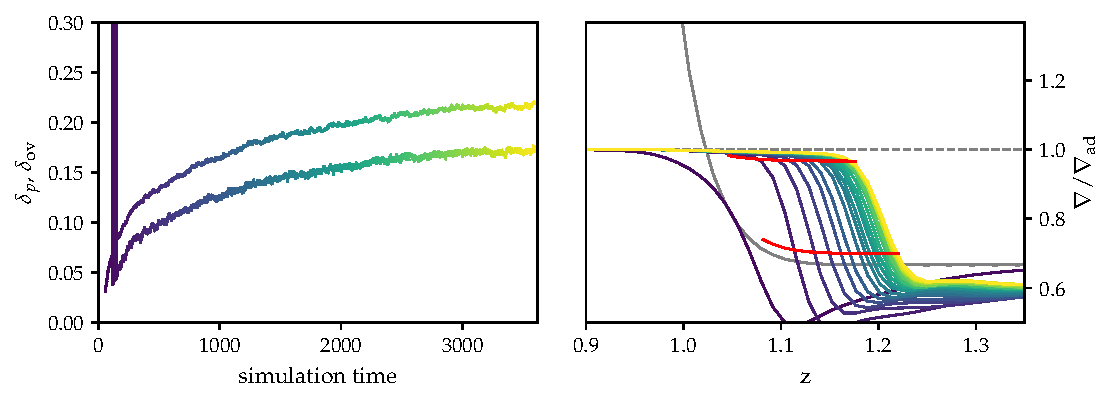
\includegraphics[width=\textwidth]{time_evolution.pdf}
\caption{
(Left top panel) Displayed is a trace of the PZ depth ($\delta_{0.5}$), normalized by the appropriate convection zone height $\tilde{L_s}$ in our simulations.
(Left middle panel) Shown is the average value of $(\justgrad - \gradrad)/\gradrad$, averaged over the full domain above $\delta_{0.5}$, as a function of time.
This provides a measure of how far out of thermal equilibrium the RZ is above the PZ, and should trend towards zero in the long-time limit.
(Left bottom panel) Shown is a rolling average over 50 freefall times of the dissipation constant $f$, defined in Eqn.~\ref{eqn:preliminary_flux_ratio}.
The vertical lines in the top and bottom panels correspond to when that measure has converged to within 1\% of its final value, where the final value is the mean taken over the last 500 freefall times of evolution shown in these plots.
(Right panel) The vertical profile of $\justgrad/\gradad$ is plotted against height at regular time intervals.
The line color denotes the time, according to the time traces in the left panels.
The constant value of $\gradad$ is denoted by the horizontal dashed grey line, and the value of $\gradrad$ is denoted by the solid grey line.
The departure points are plotted over the profile evolution ($\delta_{0.1}$ and $\delta_{0.9}$ as red lines, $\delta_{0.5}$ as black lines).
\label{fig:time_evolution}
}
\end{figure}

In Fig.~\ref{fig:time_evolution}, we show the time evolution of a Case I simulation with $\mR = 400$, $\mS = 10^3$, and $\mP_D = 4$ whose initial conditions set $\justgrad = \gradad$ in the convection zone ($z < 1$) and $\justgrad = \gradrad$ in the radiative zone ($z > 1)$.
In the top left panel, we display the extent of the penetrative region\footnote{$\tilde{L_s} = 0.8L_s$. Our choice of internal heating function (Eqn.~\ref{eqn:sim_Q}) means that the integral of $\int\Fconv$ in the convection zone is 80\% what it would be if the full $z < L_s$ region carried the full flux $F_H$, and we must appropriately account for this when measuring the overshoot depth according to Eqn.~\ref{eqn:theory_fraction}.} vs time, $\delta_{\rm{0.5}}/\tilde{L_s}$.
This region initially grows quickly over hundreds of freefall times, but this evolution slows down as the convective dynamics establish themselves and the final equilibration takes thousands of freefall times.
The steepening of $\justgrad\rightarrow\gradad$ in the growing penetrative region corresponds to a flattening of $\justgrad < \gradrad$ in the RZ above the PZ, which can be seen in the left-middle panel of Fig.~\ref{fig:time_evolution}.
In the bottom left panel of Fig.~\ref{fig:time_evolution}, we show a rolling average over 50 freefall times of the volume-averaged vorticity-based value of $f$ from Eqn.~\ref{eqn:preliminary_flux_ratio}.
Unlike the thermal stratification, this value quickly reaches a value close to its final value; for comparison, we plot grey vertical lines in the top and bottom panels of Fig.~\ref{fig:time_evolution} to indicate when each of those quantities converges to its average sampled over the last 500 freefall times displayed in that plot; we see that the dynamics converge rapidly but that the restratification is slow.
In the right panel of Fig.~\ref{fig:time_evolution}, we display the realized profile of $\justgrad/\gradad$ in our simulations at regular time intervals (where the color of the profiles corresponds to time, as in the left panels).
$\gradad$ is plotted as a dashed line while $\gradrad$ is plotted as a grey solid line.
The traces of $\delta_{0.1}$ and $\delta_{0.9}$ are plotted as red lines while that of $\delta_{0.5}$ is plotted as a black line.
We can see that the initial (fast) evolution establishes a sizeable PZ, but its final equilibration slows down (indicated by the separation between the profiles decreasing over time).
This occurs in part because the flattening of $\justgrad < \gradrad$ above the convection zone effectively increases the value of $N^2$ and thus the stiffness at the PZ-RZ boundary.

\begin{figure}[t!]
\centering
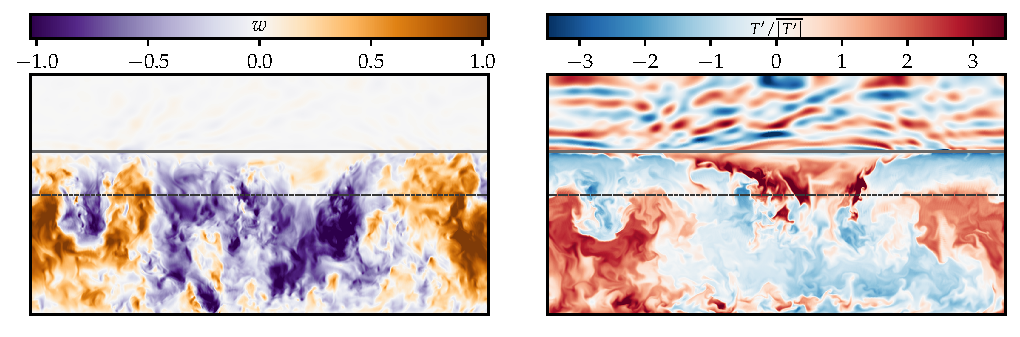
\includegraphics[width=\textwidth]{vertical_dynamics_panels.pdf}
\caption{
Displayed is an instantaneous snapshot of dynamics in a vertical slice through the simulation with $\mR = 3.2 \times 10^3$, $\mP_D = 4$ and $\mS = 10^3$.
In both panels, the nominal Schwarzschild boundary of the convection zone where $\gradad = \gradrad$ is displayed as a dashed horizontal line, and the top of the penetrative zone ($\delta_{0.1}$) is shown by a solid horizontal line.
(Left) The vertical velocity is shown; orange convective upflows extend far past the Schwarzschild boundary of the convection zone but stop abruptly where $\justgrad$ departs from $\gradad$.
(Right) Temperature fluctuations are shown, normalized by their average magnitude at each height in order to clearly display all dynamical features.
Unlike the vertical velocity, $T'$ shows distinctly different behavior in the CZ and PZ, switching sign at the Schwarzschild boundary of the convection zone.
\label{fig:vertical_dynamics_panels}
}
\end{figure}

In Fig.~\ref{fig:vertical_dynamics_panels}, we display instantaneous vertical slices through a turbulent simulation with $\mR = 3.2 \times 10^3$, $\mP_D = 4$ and $\mS = 10^3$ in an equilibrated state.
We see that strong convective dynamics (viewed in the left vertical velocity panel) extend beyond the Schwarzschild boundary of the convection zone (horizontal dashed grey line) into a penetration zone.
Above the PZ, there is a dynamically distinct stable radiative zone with negligible vertical velocity (above the solid horizontal line).
On the right, we see that hot upwellings in the convective dynamics are turned into cold upwellings in the PZ as a result of effective cooling from the sharp change in $k$ around the Schwarzschild boundary of the convection zone.
These upwellings impinge upon the stable radiative zone and excite gravity waves, but our focus in this work is on the nature of the PZ where convective velocities and temperature anomalies are oppositely signed.


\subsection{Measured penetration zone scalings}

In Fig.~\ref{fig:erf_3D_penetration_depths}, we plot measured values of the penetration depth ($\delta_{0.1}$, $\delta_{0.5}$, $\delta_{0.9}$) from Case I (discontinuous $k$) simulations.
In the left panel we plot the predicted scaling with $\mP_D$ from Eqn.~\ref{eqn:discontinuous_prediction} as well as the measured penetration depths from our simulations.
We find good agreement with the theory, and at large values of $\mP_D$ find equilibrated states in which the PZ is roughly the same size as the nominal convection zone.
%We find that the value of $\mP_D$ is the primary parameter whose value modifies the extent of the PZ.
While not presented in this work, we performed limited 2D simulations and found similar scalings, but with larger penetration zones for the same parameters in 2D than in 3D.
This signifies that $f$, and thus the viscous dissipation, is smaller in 2D than in 3D; we speculate that this is a consequence of the inverse turbulent cascade in 2D.

\begin{figure}[t!]
\centering
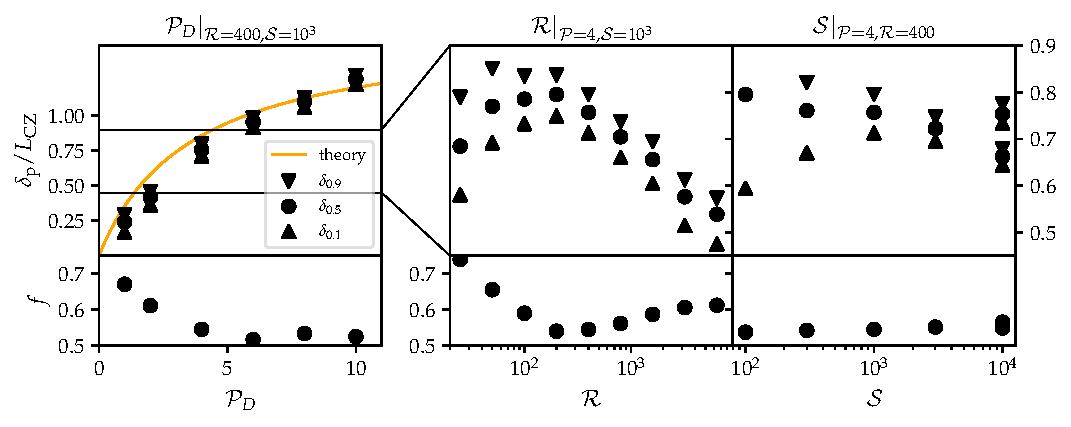
\includegraphics[width=\textwidth]{erf_3D_penetration_depths.pdf}
\caption{
Shown are penetration depths against (left) $\mP_D$, (center) $\mR$, and (right) $\mS$.
Up-triangles signify $\delta_{0.1}$, down-triangle signify $\delta_{0.9}$, and circles signify $\delta_{0.5}$.
In all panels, we plot a line corresponding to the theory of Eqn.~\ref{eqn:discontinuous_prediction}, with $f = 0.875$ and under the assumption that $f$ does not vary.
The penetration depth is a nearly linear function of $\mP_D$, in good agreement with the theory.
The black horizontal lines in the left panel represent the full vertical range of the right two panels; the effects of varying $\mS$ and $\mR$ are secondary to that of $\mP$.
In the center panel, we see that the penetration depth increases at low $\mR$ as laminar dynamics give way to time-evolving dynamics.
As we increase the turbulence, the penetration depth decreases weakly and appears to asymptote in the turbulent regime.
In the right panel, we see that the width of the transition region $\delta_{0.9} - \delta_{0.1}$, is strongly related to the stiffness.
\label{fig:erf_3D_penetration_depths}
}
\end{figure}

In the center and rightmost panels of Fig.~\ref{fig:erf_3D_penetration_depths}, we focus on modifications to the measured penetration depths achieved by varying $\mR$ (turbulence) and $\mS$ (stiffness).
We find that the penetration depth is smaller at very low (laminar) values of $\mR$ and at high (turbulent) values of $\mR$, with a peak at moderate values (for which dynamics are interesting and non-stationary, but not as turbulent as e.g., Fig.~\ref{fig:vertical_dynamics_panels}).
Our data suggest that the penetration depth, and thus the viscous dissipation, asymptotes as $\mR$ increases and so our results should be relevant for the astrophysical case in which $\mR \rightarrow \infty$ (COAUTHOR NOTE: high-$\mR$ and $\mS$ data is still preliminary, but I think that the general trends are right).
We find that mean penetration depth shows little dependence on the stiffness.
However, the depth of the transition region from the PZ to the RZ, which can be measured as $\delta_{0.9} - \delta_{0.1}$, shows a strong dependence on stiffness.
In stars, the stiffness is roughly determined by the Mach number ($\rm{Ma}^{-2} \sim \mS$), so for low-Mach stellar flows, the PZ-RZ boundary can likely be reasonably approximated as a step function in $\justgrad$.

\begin{figure}[t!]
\centering
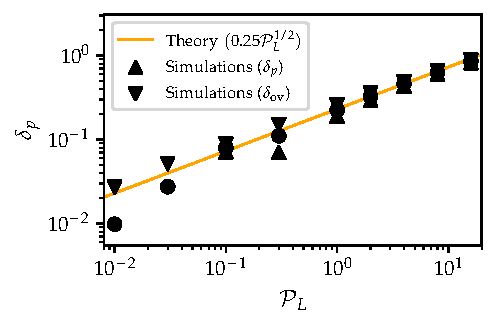
\includegraphics{linear_3D_penetration_depths.pdf}
\caption{
Similar to Fig.~\ref{fig:erf_3D_penetration_depths}, but for the Case II ``linear'' simulations where the slope of $k$ is discontinuous at the Schwarzschild point.
We plot an orange line corresponding to the theory of Eqn.~\ref{eqn:linear_prediction} with $f = 0.925$ as well as up-triangles ($\delta_{0.1}$), down-triangle ($\delta_{0.9}$), and circles ($\delta_{0.5}$).
We find that the theory describes our simulation measurements well.
\label{fig:linear_3D_penetration_depths}
}
\end{figure}

Finally, in Fig.~\ref{fig:linear_3D_penetration_depths}, we plot penetration depths as a function of $\mP_L$ for the ``linear'' Case II simulations.
We compare these depths to the theory of Eqn.~\ref{eqn:linear_prediction}.
We hold $\mR = 800$ and $\mS = 10^3$ constant for these simulations.
As in the discontinuous simulations, we find excellent agreement between the simulations and the theory.

Our simulation results present a strong case for the validity of \citet{roxburgh1989}'s integral constraint and \citet{zahn1991}'s theory of the importance of the slope of the radiative gradient near the boundary.
The generalized Eqn.~\ref{eqn:theory_fraction}, and its solution for our simulation setups in Eqns.~\ref{eqn:discontinuous_prediction} \& \ref{eqn:linear_prediction}, describe our data well.
In addition to the flux-based penetration parameter $\mP$, Eqn.~\ref{eqn:theory_fraction} depends only on a quantity related to the volume-average magnitude of the viscous dissipation comapred to the convective flux in the Schwarzschild-unstable convection zone ($f$).
In this work, from the theory lines plotted in Figs.~\ref{fig:erf_3D_penetration_depths} \& \ref{fig:linear_3D_penetration_depths}, we find
\begin{equation}
f \approx 0.875\,\,(\text{Case I: Discontinuous}),\qquad
f \approx 0.925\,\,(\text{Case II: Linear}).
\label{eqn:fit_f_values}
\end{equation}
In both cases, $f$ is a parameter of order 0.9.
With these results as an initial guess for the magnitude of $f$, Eqn.~\ref{eqn:theory_fraction} can be straightforwardly used to implement these penetrative zones in a 1D stellar structure code.

\section{A modified solar model}
\label{sec:solar_model}
We now examine briefly how our theory modifies a simple structure model of the Sun.
We implement a simple prescription of convective penetration in MESA \citep{paxton_etal_2013} as follows:
\begin{enumerate}
\item Find the radial location of the radiative-convective boundary according to the Schwarzschild criterion, $r_{\rm{RCB}}$.
Also evaluate the value of the mixing length $\ell$ at that location.
\item Integrate the magnitude of the convective luminosity within the convection zone, $L_{\rm{CZ}} = \int_{r_{\rm{RCB}}}^{r_{\rm{RCB}} + \ell} L_{\rm{conv}} dr$.
\item Following Eqn.~\ref{eqn:theory_fraction} and the measured values for $f$ in Eqn.~\ref{eqn:fit_f_values}, integrate $L_{\rm{PZ}} = \int_{r_{\rm{RCB}}}^{r_{\rm{RCB}} + \delp} (L_{\rm{rad}} - L_{\rm{rad,ad}}) dr$, where $L_{\rm{rad}}$ is the radiative luminosity carried by $\gradrad$ and $L_{\rm{rad,ad}}$ is the radiative luminosity carried by $\gradad$.
We determine the value of $\delp$ according to Eqn.~\ref{eqn:theory_fraction} so that
\begin{equation}
L_{\rm{PZ}} = (1 - f)L_{\rm{CZ}},
\label{eqn:mesa_equation}
\end{equation}
with an initial guess of $f = 0.9$.
\item Override the value of $\justgrad$ in the MESA solver to set $\justgrad = \gradad$ from $r_{\rm{RCB}}$ to $r_{\rm{RCB}} - \delta_p$.
\item Mix within this new convection zone by setting the convective velocities according to the average convective luminosity in the penetration zone, $4\pi r^2 \rho v^3 \sim L_{\rm{PZ}}$.
\end{enumerate}

TODO: Implement this in MESA, and make a simple figure comparing some solar profiles near the base of the CZ!

We find a convection zone which extends an additional $X H_p$ beneath the nominal Schwarzschild base of the convection zone.
This results in a discontinuous temperature profile, which would result in an acoustic ``glitch'' on the solar frequencies.
Past work has suggested from observations that the maximum depth of such an extended adiabatic region should be limited to $0.05 H_p$, which is smaller than what is found in our model \citep[see e.g., section 7.2.1 of][]{basu2016}.
However, our results here are in line with the recent simulations of \citet{kapyla2019}, which suggest an overshooting depth of $0.2 H_p$ at the base of the solar convection zone.


\section{Discussion}
\label{sec:discussion}
In this work, we used \citet{roxburgh1989}'s integral constraint and flux-based argument analagous to \citet{zahn1991}'s theory to derive a parameterization of convective penetration according to the convective flux and viscous dissipation.
We designed and analyzed two sets of simulations which showed good agreement with that theoretical parameterization.
We furthermore examined briefly what the impliciations of this theory could be for a simple solar model.
Our results suggest that stellar convection zones should be bounded by appreciably large penetration zones.
In extreme cases, we observe penetration zones which are as large as the convection zones they accompany; however, for realistic stellar values ($\mP \approx 1$), we find that they may be as large as 20-30\% of the convective zone length scale (the mixing length).

The simulations we presented in this work were the simplest possible simulations to try to test the basic tenents of \citet{roxburgh1989} and \citet{zahn1991}'s theory.
In particular, they demonstrate that indeed the shape of the flux near the convective boundary and the viscous dissipation together fully determine the depth of the penetration zone.
The precise value of $f$ achieved in natural, turbulent, fully compressible, spherical stellar convection may be different from the value of $f \approx 0.9$ measured in this work.
Future work should aim to determine how much the values in Eqn.~\ref{eqn:fit_f_values} vary when these more realistic effects are taken into account.

Furthermore, it is important to note that stellar opacities, and thus stellar conductivities, are functions of thermodynamic variables rather than radial location.
As a result, the formation of a penetration zone will in turn affect the conductivity profile and $\gradrad$, which will in turn affect the estimate of how deep a penetration zone should form.
Future studies should follow e.g., \citet{kapyla_etal_2017} and implement realistic opacity profiles which evolve self-consistently with the thermodynamic state in order to understand how these effects feedback into one another.

An additional complication is that stellar fluid dynamics exist in the regime of Pr$\,\ll1$ \citep{garaud2021}.
Dynamics in this regime may be different from those in the regime of Pr $\lesssim 1$ that we studied here, which in theory could affect $f$.
Recently, \citet{kapyla2021} found that convective flows exhibited more penetration at low Pr than high Pr.
Future work should aim to understand whether $f$ depends strongly on $\Pran$ in the turbulent regime.

Two other interesting complications in stellar contexts are rotation and magnetism.
In the rapidly rotating limit, rotation creates quasi-two-dimensional flows, which could affect the length scales on which dissipation acts and thus modify $f$.
Furthermore, magnetism adds an additional ohmic dissipation term, which could in theory drastically change our hydrodynamical measurement of $f \approx 0.9$.

Finally, we note that our work here assumes a uniform composition through the convective and radiative region.
Frequently within stars, convective boundaries coincide with discontinuities in composition profiles \citep{salaris_cassisi_2017}.
Future work should also aim to determine if stabilizing composition gradients can prevent the formation of penetration zones seen here (as in Fig.~\ref{fig:time_evolution}).

In summary, we have unified \citet{roxburgh1989}'s integral constraint with \citet{zahn1991}'s theory of flux-dependent penetration into a parameterized theory of convective penetration.
We tested this theory with simulations and found good agreement between the theory and our simulations.
In future work, we will aim to more robustly implement this theory into MESA and test some of the complicating factors we discussed here.





\begin{acknowledgments}
We'd like to thank Keaton Burns and Kyle Augustson for useful discussions which improved the content of this manuscript.
TODO thank Nordita program.
EHA is funded as a CIERA Postdoctoral fellow and would like to thank CIERA and Northwestern University. 
Computations were conducted with support from the NASA High End Computing (HEC) Program through the NASA Advanced Supercomputing (NAS) Division at Ames Research Center on Pleiades with allocation GID s2276.
\end{acknowledgments}


\appendix

\section{Accelerated Evolution}
\label{app:accelerated_evolution}
As demonstrated in Fig.~\ref{fig:time_evolution}, the time evolution of simulations which start from a state based on the Schwarzschild criterion can be prohibitively long.
In \citet{anders_etal_2018}, we explored the long time evolution of simple convective simulations and found that fast-forwarding the evolution of a convective simulation's internal energy and thermal structure can be done accurately.
This can be done because the convective dynamics converge rapidly even if the thermal profile converges slowly.
This same separation of scales is observed in the top and bottom left panels of Fig.~\ref{fig:time_evolution} in this work, and so similar techniques should be applicable.

In this work, we accelerate the evolution of of our simulations in order to more quickly determine the final size of the evolved penetration zones according to the following algorithm.
\begin{enumerate}
\item Once a simulation has a volume-averaged Reynolds number greater than 1, we wait 10 freefall times to allow dynamical transients to pass.
\item We measure the departure points ($\delta_{0.1}$, $\delta_{0.5}$, $\delta_{0.9}$) every freefall time, and store this information for 30 freefall times.
\item We linearly fit each of the departure points' evolution against time using NumPy's \texttt{polyfit} function.
We assume that convective motions influence $\delta_{0.1}$ and $\delta_{0.5}$ more strongly than $\delta_{0.9}$.
We measure the time-evolution of the convective front $\frac{d \delp}{dt}$ by averaging the slope of the linear fits for $\delta_{0.1}$ and $\delta_{0.5}$.
\item We take a large ``time step'' of size $\tau_{\rm{AE}}$ forward.
We calculate $\Delta \delta_p = \tau_{\rm{AE}} \frac{d \delp}{dt}$.
\begin{itemize}
\item If $\Delta \delta_p < 0.005$, we erase the first 15 time units worth of departure point measures and return to step 2 for 15 time units.
\item  If $\Delta \delta_p$ is large, we adjust the top of the PZ by setting $\delta_{0.5,\rm{new}} = \angles{\delta_{0.5}}_t + \Delta \delta_p$ (angles represent a time average).
If $|\Delta \delta_p| > 0.05$, we limit its value to 0.05.
We calculate the width of the thermal adjustment layer $d_w$ as the minimum of $\angles{\delta_{0.9} - \delta_{0.5}}_t$ and $\angles{\delta_{0.5} - \delta_{0.1}}_t$.
We adjust the mean temperature gradient to
\begin{equation}
\partial_z \overline{T} = -\gradad - H(z; \delta_{\rm{0.5,\rm{new}}}, d_w) \Delta\justgrad,
\label{eqn:initial_grad}
\end{equation}
where $H$ is defined in Eqn.~\ref{eqn:heaviside} and $\Delta\justgrad = \gradrad - \gradad$.
We also multiply the temperature perturbations and full convective velocity field by $(1 - H(z; 1, 0.05))$.
This sets all fluctuations above the nominal Schwarzschild convection zone to zero, thereby avoiding any strange dynamical transients caused by the the old dynamics at the radiative-convective boundary (which has moved as a result of this process).
\end{itemize}
\item We restart from step 1.
\end{enumerate}
In general, we start our simulations with an initial profile according to Eqn.~\ref{eqn:initial_grad} with a value $\delta_{0.5,\rm{new}} \geq 0$.
If a simulation returns to step 2 from step 4 ten times over the course of its evolution, we assume that it has converged near its answer, stop this iterative loop, and allow the simulation to timestep normally.
Additionally, in some simulations, we ensure that this process occurs no more than 25 times.
This process effectively removes the long diffusive thermal evolution on display in the middle left panel of Fig.~\ref{fig:time_evolution} by immediately setting the mean temperature profile to the radiative profile above the PZ.

In Fig.~\ref{fig:AE_time_figure}, we display the time evolution of $\delp/\tilde{L_s}$ and $\angles{f}$ in the $\mP_D = [1,2,4]$ simulations using black lines.
We overplot the evolution of simulations which use this accelerated evolution procedure using orange and green lines.
For the orange-line simulations, we use initial conditions which specify a value of $\delp$ that is smaller than the expected evolved value of $\delp$.
For the purple-line simulations, we use initial conditions which specify a value of $\delp$ that is larger than the expected evolve value.
Regardless of our choice of initial condition, we find that this AE procedure quickly evolves our simulations to within a few percent of the final value.
If these simulations are not in a stationary state after this procedure, we timestep them straightforwardly until we are satisfied that they have converged.

\begin{figure}[t!]
\centering
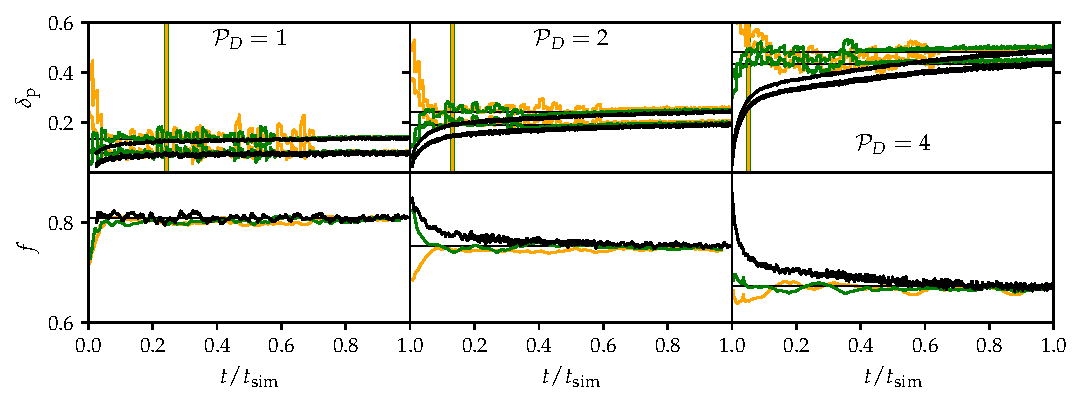
\includegraphics[width=\textwidth]{AE_time_figure.pdf}
\caption{
\label{fig:AE_time_figure}
(top row) Time traces of $\delta_p/\tilde{L_s}$ for simulations which are computed using (black lines) standard timestepping, (green lines) accelerated evolution with large initial values of $\delp$, and (orange lines) accelerated evolution with small initial values of $\delp$.
Accelerated evolution timesteps can be see as discontinuities in the $\delp/\tilde{L_s}$ trace.
Once the procedure gets to within a few percent of the appropriate value, any large steps away from the ``correct'' solution are quickly reversed.
(Bottom row) Same as top row, but where $\angles{f}$ is being shown.
}
\end{figure}



\section{Table of simulation parameters}
\label{app:simulation_table}





\bibliographystyle{aasjournal}
\bibliography{biblio}
\end{document}
